\chapter{Dicom-Presenter Rendering Engine}
\vspace{-10mm}
Dicom-Presenter as firstly designed in work \cite{neskudla} was an application depending on cca eight external libraries. The libraries dependency complicated application compilation and deployment. All the libraries must be executable on a target machine.

Therefore, a valuable task was to remove some of the library dependencies. Most of the deployment complications were related to OpenGL library. Next to OpenGL itself, GLEW, Cg toolkit and plib libraries were used to extend OpenGL functionality. All the libraries need to be hardware and software supported on the target machine\footnote{The OpenGL library requires GPU drivers supporting the library to be installed on the target machine. GLEW library require the GPU to support spatial textures (among others). Cg toolkit library requires the GPU to support pixel shader. Moreover, the Cg toolkit library requires a hardware-dependent configuration during the compilation time or at run time.}. Hence, removing OpenGL library with all three dependencies would contribute to application deployability.

The OpenGL library was connected to nine of all twenty-six Dicom-Presenter modules. Global OpenGL function were called within the modules considering previous OpenGL function calls done in another modules. Therefore, removing the OpenGL library from the application is a significant intervention to the existing source code. To understand the new non-OpenGL implementation, it is mandatory to be familiar with application object model.

\section{Dicom-Presenter Object Model}

Dicom-Presenter consists of twenty six modules, together making 5000 lines. Each module includes one class (rarely two classes). The classes can be divided into two groups: classes which represent some visible element (image, workspace, ...) and classes which maintain only abstract functionality.

To understand the hierarchical arrangement of application classes, the following passages describe three views on the object model:

\begin{itemize}
\item Rendering the visual content. All the classes related to some visible element must be sequentially called to paint their content to buffer container.
\item Control events forwarding. Each captured pointing device event must be forwarded to the object to which it belongs.
\item Image storing. A view on the object model related to the classes maintaining abstract functionalities can start with the actions attached to loading an image from hard disk.
\end{itemize}

\subsection{Dicom-Presenter Object Model Description}
As was said in \ref{dicom-presenter}, Dicom-Presenter application window consists of following elements:  Workspace, Image Explorer, Workspace Explorer and Info Panel. The Workspace acts as a main graphic output, it is used for viewing DICOM images. To ensure usability of Dicom-Presenter during presentations, several workspace sessions can be opened at the same time. Therefore, Workspace Explorer acts as a switch among opened workspaces\footnote{The process is similar as workspaces switching in GNOME/KDE.}. Due to the fact that an image can be opened at a number of workspaces at once, Image Explorer is used to manage opened images. Info Panel holds information about the opened image or the opened workspace.

\begin{figure}
	\caption{Dicom-Presenter classes representing a visible element.}
	\begin{center}
	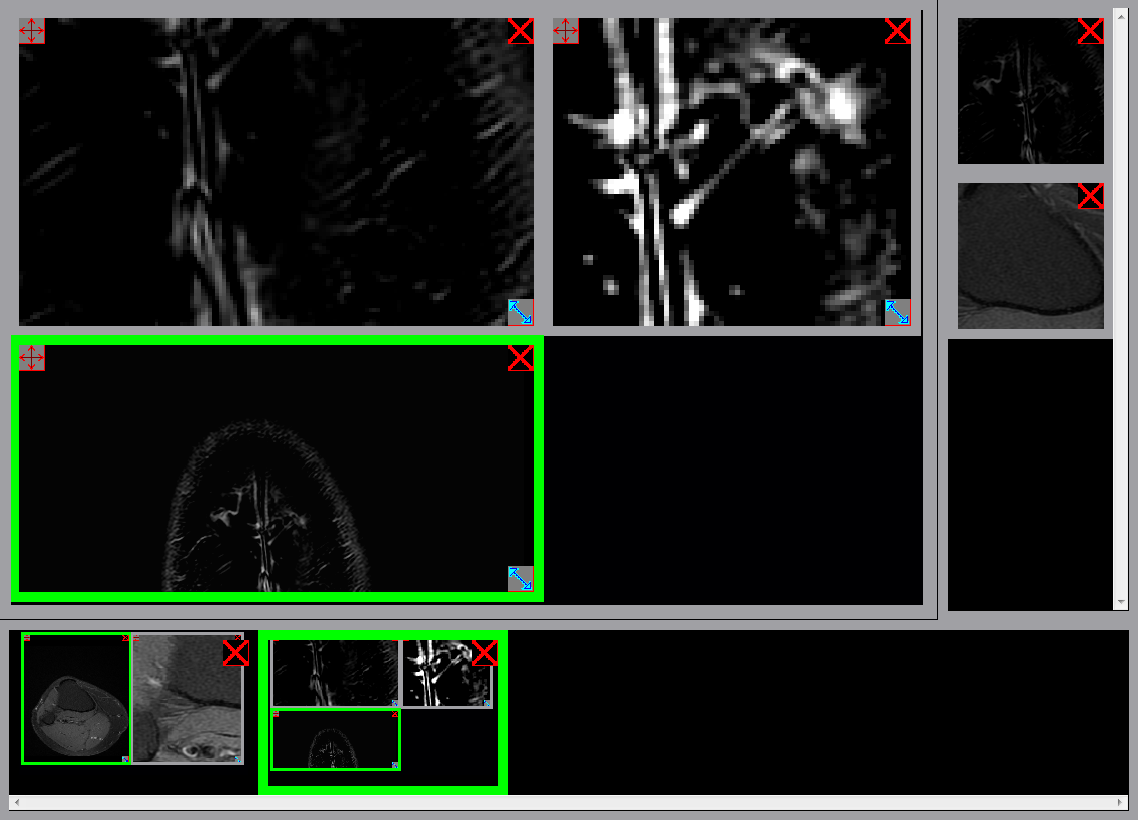
\includegraphics[width=\textwidth]{Text/IMG/dicom-presenter-gui.png}
	\end{center}
	\label{paint}
\end{figure}

\subsection{Graphic Output Rendering in Dicom-Presenter}
\label{renderingprocess}
The mentioned control elements of Dicom-Presenter: Image Explorer and Workspace Explorer are rendered manually. They are not based on existing Qt library class. Thus, if a graphic output of Dicom-Presenter is rendered all classes representing some graphic element must be called. 

An impulse to render the graphic window can be called at any time from any part of the application. A static function is used to obtain the pointer to output window, then a function called \clist{paint} is called.

The \clist{paint} function of main window object (\clist{CWidget}) then calls paint functions of all elements present in the window: an active Workspace, Workspace Explorer and Image Explorer. All the elements contain smaller subelements. The Workspace calls paint functions of all images present appearing on the Workspace, Workspace Explorer calls paint functions of all images containing workspace previews and finally the Image Explorer calls paint functions of all images operated by it. A schema of the process can be seen on Figure \ref{paint}.
\begin{comment}
\begin{lstlisting}[label=cwidgetpaint,caption={Sequentionally rendering each visible element.},escapeinside={@}{@}]
void CWidget::paint() {
	...
	CWorkspaceManager::GetInstance()->GetActiveWorkspace()->paint(...);
	CImageExplorer::GetInstance()->paint(...);
	CWorkspaceExplorer::GetInstance()->paint(...);
	...
}
void CWorkspace::paint(...) {
	...
	while (images.hasNext()) {
	  ...
		cimage->paint(...);
		...
	}
	...
}
void CImageExplorer::paint(...) {
	...
	while (images.hasNext()) {
		...
		cimage->paint(...);
		...
	}
	...
}
void CWorkspaceExplorer::paint(...) {
	...
	while (workspaces.hasNext()) {
		...
		snap.paint(painter);
		...
	}
	...
}
\end{lstlisting}
\end{comment}

\begin{figure}
	\caption{A hierarchy of classes presenting paintable elements.}
	\begin{center}
	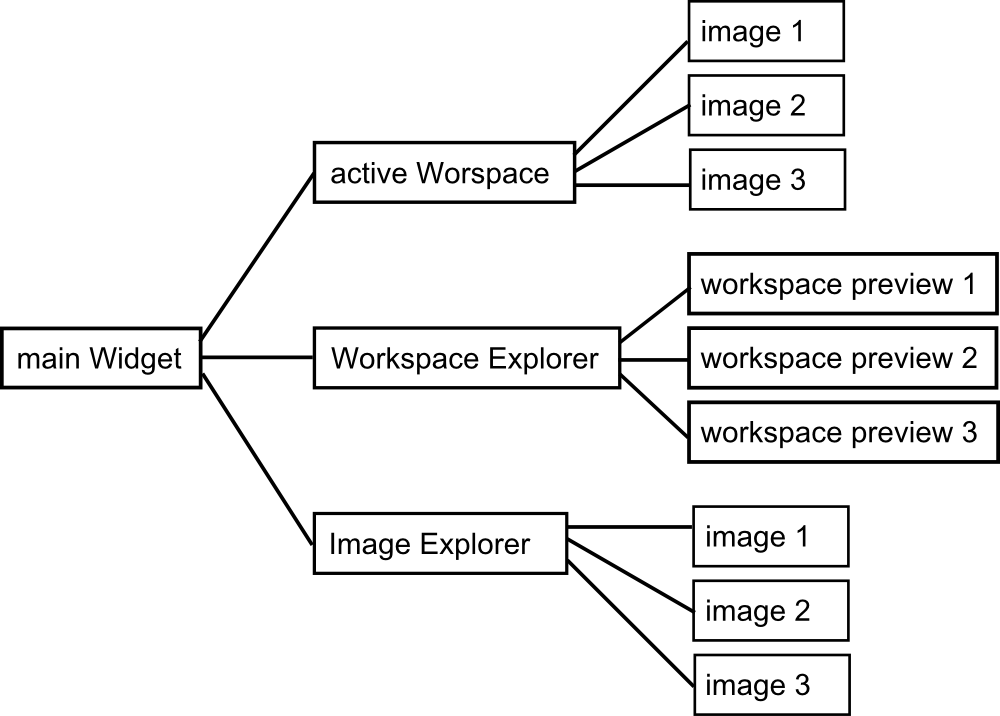
\includegraphics[width=\textwidth]{Text/IMG/paint.png}
	\end{center}
	\label{paint}
\end{figure}

\subsection{Control Event Forwarding in Dicom-Presenter}

Similarly as the paint directions are distributed to the application classes, pointing device events are distributed through the object model. As was said in previous section, all the visible elements of Dicom-Presenter visual output are rendered manually. Therefore, if the user performs some pointing device action on some visible element (wheel-scroll, mouse-click, etc.), the event must be manually forwarded to the related object.

Pointing device events in Dicom-Presenter can be divided into two groups: events starting an action and events related to a previously started action. Mouse click and mouse double click start an action, mouse move and wheel scroll are related to previous event. If a click or double-click event is captured, then the process of finding the related object must be started. If a mouse move or wheel scroll are received, the event is instantly forwarded to the last used object.

The process of finding the object related to click or double-click event is similar to the painting process. The main widget receives a click event together with the position of the mouse pointer in coordinates related to the widget. Each of all three parent elements on the widget (Workspace, Workspace Explorer and Image Explorer) have saved their position in the main widget. Therefore, the main widget asks all three elements if the mouse pointer position corresponds with their position. The element giving positive response receives the event.

If the active Workspace receives the event, then it must be decided which of the opened images is related to the action. Thus, all displayed images are iteratively asked whether their location cover the pointer position. Then, the event is forwarded to the prospective image. The image object performs required task such as move, zoom or brightness change.

Similarly, if the mouse pointer was not located on the active Workspace but on the Workspace Explorer or the Image Explorer, then, the event is redirected to the appropriate object. Afterwards, the object iterates through its owned objects and finds the one related to the event received (workspace preview or image preview). The desired action can be performed.

The schema is different from usual GUI programming techniques where some GUI framework would be used. The framework solves event redirecting itself, as seen in Section \ref{guiframeworks}.

\subsection{Image Opening in Dicom-Presenter}

Another view to application object model can be described by following actions done, when opening an image. When a user gives a direction to open a DICOM study, at first the Image Explorer is called. Image Explorer creates a new object of Image type. The new Image object calls a 3DTextureManager object to create a new object representing a three-dimensional texture (dicom3DTexture). Then an object of DCMTK library is created to load the data from the hard disk. The object allows decompressing the data and saving them into computer memory in a format mentioned in Section \ref{rawdata}.

\section{Rendering Engine Implementation}

In the first version of Dicom-Presenter, all the rendering was solved with use of OpenGL library. OpenGL global functions could be called anywhere in the application and the OpenGL output was directed to the computer screen instantly. To access images in GPU memory, OpenGL uses integer numbers as handlers. A DICOM study was saved into GPU memory in CDicom3DTexture class and obtained from GPU memory inside a Image class using proper handler (See page 19 in \cite{flaska_bc}).

Qt library uses object-oriented approach to perform image rendering (see Section \ref{renderingprocess}). The rendering process starts in main window - active Workspace, Image Explorer and Workspace Explorer objects are called to draw their content - a \clist{QPainter} object is passed to them. The \clist{QPainter} object is used for redirecting the graphic output to a target pixel map. All the three objects then call all owned subobjects and redirect the \clist{QPainter} object to them.

As was described in Section \ref{rendering}, \clist{QPixmap} class is optimized for rendering, \clist{QImage} class is optimized for pixel manipulation. Therefore, images are stored in \clist{QImage} objects and the output is drawed into a \clist{QPixmap} object.

\begin{lstlisting}[language=,escapeinside={@}{@},morekeywords={zzz,ADD_EXECUTABLE,add_custom_command,add_library,target_link_libraries,OUTPUT,COMMAND,xxx})]
void CWidget::paint(){
  QPixmap *outputpixmap = new QPixmap(this->width(),this->height());
  QPainter *@\red{qpainter}@ = new QPainter();
  @\red{qpainter}@->begin(outputpixmap);
  if (CWorkspaceManager::GetInstance()->GetActiveWorkspace()) {
    QRect position(...);
    CWorkspaceManager::GetInstance()->@\orange{GetActiveWorkspace()->paint}@(@\red{qpainter}@,position);
  }
  CImageExplorer::GetInstance()->paint(@\red{qpainter}@);
  CWorkspaceExplorer::GetInstance()->paint(@\red{qpainter}@);
  setPixmap(*outputpixmap);
  repaint(); 
 ...
}
\end{lstlisting}

\begin{lstlisting}[language=,escapeinside={@}{@},morekeywords={zzz,ADD_EXECUTABLE,add_custom_command,add_library,target_link_libraries,OUTPUT,COMMAND,xxx})]
void @\orange{CWorkspace::paint}@(QPainter* @\red{qpainter}@, QRect position){
  QPixmap* @\lightblue{workspacepixmap}@ = new QPixmap(iSize.x(),iSize.y());
  QListIterator<CImage*> images(iImages);
  while(images.hasNext()){
    CImage *cimage = images.next();
    QPainter *qpainter2 = new QPainter();
    qpainter2->begin((QPaintDevice*)@\lightblue{workspacepixmap}@);
    cimage->paint(qpainter2);
    if(iActiveImage==cimage){
      cimage->DrawSelection(qpainter2);
    }
    ...
  }
  @\red{qpainter}@->drawPixmap(position,*@\lightblue{workspacepixmap}@);
  DrawBorderRect(@\red{qpainter}@);
  ...
}
\end{lstlisting}